\documentclass[aspectratio=169,11pt]{beamer}
\usepackage[T1]{fontenc}
\usepackage{lmodern}
\usepackage{booktabs}
\usepackage{tikz}
\usetikzlibrary{arrows.meta,positioning,shapes.geometric}
\usepackage{pgfplots}
\pgfplotsset{compat=1.16}

\definecolor{navy}{HTML}{16324F}
\definecolor{teal}{HTML}{1B7F79}
\definecolor{amber}{HTML}{D98E04}
\definecolor{brick}{HTML}{B23A48}
\definecolor{paper}{HTML}{F7F9FB}

\usetheme{default}
\usecolortheme{default}
\setbeamercolor{background canvas}{bg=paper}
\setbeamercolor{title}{fg=navy}
\setbeamercolor{frametitle}{fg=navy}
\setbeamercolor{structure}{fg=teal}
\setbeamercolor{itemize item}{fg=teal}
\setbeamercolor{itemize subitem}{fg=teal}
\setbeamercolor{block title}{bg=navy,fg=white}
\setbeamercolor{block body}{bg=white,fg=black}
\setbeamercolor{alerted text}{fg=brick}
\setbeamerfont{frametitle}{series=\bfseries,size=\Large}
\setbeamertemplate{navigation symbols}{}
\setbeamertemplate{frametitle}{%
  \vskip1.2ex\usebeamercolor[fg]{frametitle}\usebeamerfont{frametitle}\insertframetitle\par
  \vskip-0.4ex{\color{teal}\rule{\textwidth}{1.2pt}}}
\setbeamertemplate{footline}{%
  \hfill\color{gray}\scriptsize IT418 Cloud Computing \quad\insertframenumber/\inserttotalframenumber\hspace{2mm}\vspace{1.5mm}}
\setbeamertemplate{itemize items}[circle]

\title{Unified Detection of Tenant-Isolation Violations and QoS Fairness Breaches in Multi-Tenant Kubernetes}
\author{H S Jayanth (231IT024) \and Suvarna G (231IT077)}
\institute{IT418 --- Cloud Computing}
\date{}

\begin{document}

\begin{frame}[plain]
\vspace{8mm}
{\color{navy}\Large\bfseries Unified Detection of Tenant-Isolation Violations\\and QoS Fairness Breaches in Multi-Tenant Kubernetes\par}
\vspace{4mm}
{\color{teal}\rule{0.45\textwidth}{1.5pt}}\par\vspace{4mm}
\large H S Jayanth (231IT024) \quad Suvarna G (231IT077)\par
\vspace{1mm}\normalsize IT418 --- Cloud Computing, course project\par
\vspace{8mm}
\small One pipeline for the two ways a shared cluster fails its tenants: \alert{security} (isolation) and \alert{performance} (noisy neighbor).
\end{frame}

\begin{frame}{The problem: shared clusters fail tenants in two ways}
\begin{columns}[T]
\column{0.5\textwidth}
\begin{block}{Isolation violation (security)}
Tenant A improperly reaches Tenant B's resources: a bad RoleBinding, a missing NetworkPolicy, a misused credential.
\end{block}
\column{0.5\textwidth}
\begin{block}{Fairness violation (performance)}
Tenant A's workload starves Tenant B: slow responses with \emph{no} security rule broken. The ``noisy neighbor''.
\end{block}
\end{columns}
\vspace{3mm}
\begin{itemize}
\item A control-plane monitor sees \emph{who asked for what}, but is blind to a CPU hog that makes no illegal call.
\item An eBPF network monitor sees cross-namespace flows, but not cgroup CPU throttling.
\item \alert{No tool fuses both, and none is evaluated quantitatively across both.}
\end{itemize}
\end{frame}

\begin{frame}{Base paper and the gap}
\textbf{Shamim, Hu, Rahman --- DAST for Kubernetes (FSE '25).} Dynamic testing finds thousands of CIS violations that static analysis missed.
\vspace{2mm}
\begin{columns}[T]
\column{0.5\textwidth}
\textbf{Limitations we address}
\begin{itemize}
\item no implemented tool
\item security-only; ignores fairness
\item no precision / recall / latency
\item control-plane signals only
\end{itemize}
\column{0.5\textwidth}
\textbf{Our contribution}
\begin{itemize}
\item working multi-source pipeline
\item fairness requires an \alert{independent victim-side} breach
\item 8 repeatable scenarios + negative controls
\item honest evaluation, including what went wrong first
\end{itemize}
\end{columns}
\end{frame}

\begin{frame}{Architecture: three monitors, one fusion layer}
\centering
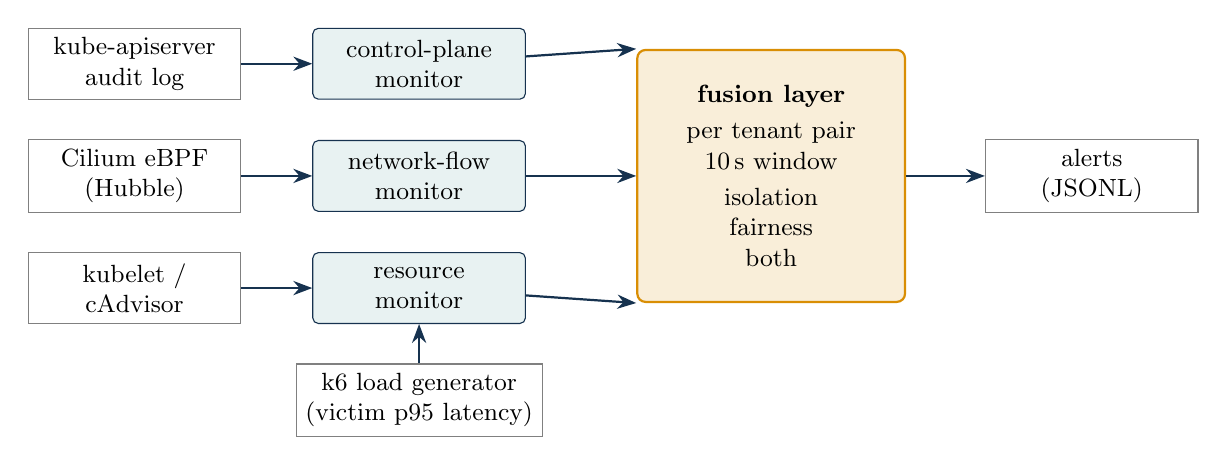
\begin{tikzpicture}[
  node distance=5mm and 9mm,
  box/.style={draw=navy, rounded corners=2pt, align=center, minimum height=9mm, minimum width=27mm, font=\small, fill=teal!10},
  src/.style={draw=gray, align=center, minimum height=9mm, minimum width=27mm, font=\small, fill=white},
  fus/.style={draw=amber, thick, rounded corners=3pt, align=center, minimum height=32mm, minimum width=34mm, font=\small, fill=amber!15},
  arr/.style={-{Stealth[length=2.4mm]}, thick, navy}]
\node[src] (audit) {kube-apiserver\\audit log};
\node[src, below=of audit] (cil) {Cilium eBPF\\(Hubble)};
\node[src, below=of cil] (kub) {kubelet /\\cAdvisor};
\node[box, right=of audit] (cpm) {control-plane\\monitor};
\node[box, right=of cil] (nfm) {network-flow\\monitor};
\node[box, right=of kub] (rm) {resource\\monitor};
\node[src, below=of rm] (k6) {k6 load generator\\(victim p95 latency)};
\node[fus, right=14mm of nfm] (fusion) {\textbf{fusion layer}\\[2pt]per tenant pair\\10\,s window\\[2pt]isolation\\fairness\\both};
\node[src, right=10mm of fusion] (alerts) {alerts\\(JSONL)};
\draw[arr] (audit) -- (cpm);
\draw[arr] (cil) -- (nfm);
\draw[arr] (kub) -- (rm);
\draw[arr] (k6) -- (rm);
\draw[arr] (cpm) -- (fusion.north west);
\draw[arr] (nfm) -- (fusion);
\draw[arr] (rm) -- (fusion.south west);
\draw[arr] (fusion) -- (alerts);
\end{tikzpicture}
\vspace{1mm}

\small Hubble's eBPF probes sit at the network layer, so resource pressure needs its own collector.
\end{frame}

\begin{frame}{Fusion rules (deterministic, easy to validate)}
\begin{enumerate}
\item[\alert{1}] \textbf{Isolation:} any cross-namespace control-plane or network-flow event is sufficient on its own.
\item[\alert{2}] \textbf{Fairness:} resource pressure in tenant A \alert{and} a latency breach in tenant B, overlapping in time. Elevated usage alone is never enough.
\item[\alert{3}] \textbf{Both:} an isolation and a fairness cluster for the same tenant pair that overlap are merged.
\end{enumerate}
\vspace{3mm}
\begin{block}{Why require the victim-side signal?}
A tenant legitimately using more CPU is not a violation. Without an independent measure of harm, a pressure-only rule flags every busy tenant.
\end{block}
\end{frame}

\begin{frame}{Testbed and static baseline}
\begin{columns}[T]
\column{0.52\textwidth}
\textbf{Testbed}
\begin{itemize}
\item kind cluster, Cilium + Hubble, API audit log
\item 3 tenant namespaces, each with scoped RBAC, default-deny NetworkPolicy, ResourceQuota + LimitRange
\item boundaries verified: cross-ns API call denied, flow dropped, over-quota pod rejected
\item Trivy CI gate on HIGH/CRITICAL
\end{itemize}
\column{0.46\textwidth}
\textbf{kube-bench (CIS 1.9)}\par\vspace{1mm}
\small
\begin{tabular}{lrrr}
\toprule
 & PASS & FAIL & WARN\\
\midrule
Master & 40 & 7 & 12\\
Node & 16 & 2 & 6\\
Policies & 2 & 4 & \alert{29}\\
\midrule
Total & 66 & 13 & 51\\
\bottomrule
\end{tabular}
\vspace{1mm}

\footnotesize It can say a control \emph{should} be checked, not that the policy is correct and in force at runtime.
\end{columns}
\end{frame}

\begin{frame}{Evaluation design}
\begin{columns}[T]
\column{0.5\textwidth}
\textbf{8 scenarios $\times$ 5 repetitions}
\begin{itemize}
\item \emph{Isolation (5):} NetworkPolicy misconfig, RBAC over-permission, credential misuse, privilege escalation, data-plane-only crossing
\item \emph{Fairness (3):} CPU hog, memory pressure, quota bypass
\end{itemize}
\column{0.5\textwidth}
\textbf{10 negative controls}
\begin{itemize}
\item 5 \emph{idle} windows
\item 5 \emph{benign-busy} windows: a well-behaved tenant saturating its own small CPU limit
\end{itemize}
\vspace{2mm}
\small Idle windows can't tell naive from fused rules apart: neither fires on silence.
\end{columns}
\vspace{3mm}
Detector configs: control-plane-only, network-flow-only, \textbf{fused-isolation}; pressure-only, \textbf{fused-fairness}.
\end{frame}

\begin{frame}{Finding 1: on a big host, the noisy neighbor wasn't noisy}
\begin{itemize}
\item First sweep: fused-fairness scored \alert{0 / 15}. The rule was correct; its evidence never existed.
\item Replaying victim latency: p95 $\approx$ 3.6\,ms \emph{before and during} every injection. CFS-limited hogs on a 16-core host can't hurt a trivial handler.
\end{itemize}
\vspace{2mm}
\begin{block}{Fix: make the contention real}
Pin the worker to a 2-CPU cpuset; run hogs on the victim's node; scale them (6$\times$200m, memory-ramping pods, a multi-process quota-bypass hog).\\
Victim p95: \textasciitilde 5.7\,ms $\to$ 17--95\,ms.
\end{block}
\small This is engineered contention, and a result in itself: per-container CPU limits protected co-located tenants well.
\end{frame}

\begin{frame}{Isolation: the two signals are complementary}
\begin{columns}[c]
\column{0.55\textwidth}
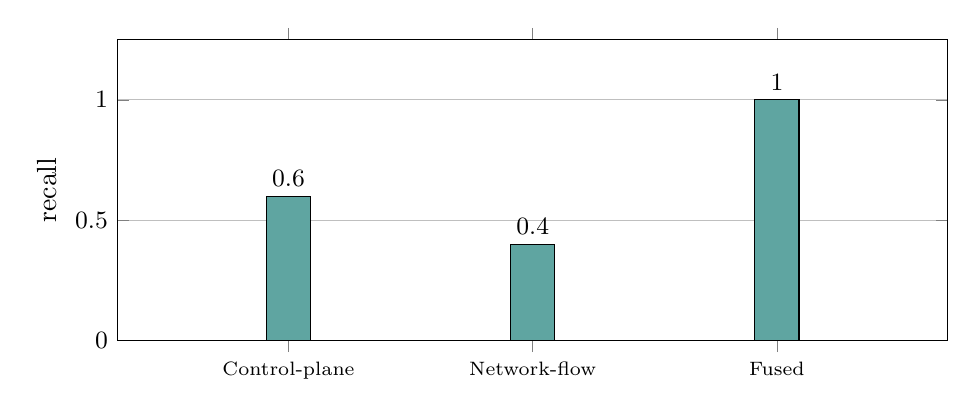
\begin{tikzpicture}
\begin{axis}[ybar, width=\textwidth, height=5.4cm, ymin=0, ymax=1.25, bar width=16pt, xticklabel style={font=\scriptsize},
  symbolic x coords={Control-plane,Network-flow,Fused}, xtick=data, ylabel={recall},
  nodes near coords, nodes near coords style={font=\small}, tick label style={font=\small},
  enlarge x limits=0.35, ymajorgrids]
\addplot[fill=teal!70] coordinates {(Control-plane,0.60)(Network-flow,0.40)(Fused,1.00)};
\end{axis}
\end{tikzpicture}
\column{0.43\textwidth}
\begin{itemize}
\item Control-plane misses NetworkPolicy and data-plane-only runs: no API call.
\item Network-flow misses RBAC, credential and privilege runs: no cross-tenant flow.
\item \alert{Fused: 25/25, zero false positives.}
\end{itemize}
\end{columns}
\end{frame}

\begin{frame}{Finding 2: idle controls hid a precision problem}
\small
\begin{center}
\begin{tabular}{lcccc}
\toprule
Fairness config & TP/FN & FP idle/busy & Precision & Latency\\
\midrule
pressure-only & 15/0 & 0/3 & 0.83 & 13.5\,s\\
fused @ 1.5$\times$ & 13/2 & 0/\alert{5} & \alert{0.72} & 2.5\,s\\
\bottomrule
\end{tabular}
\end{center}
\normalsize
\begin{itemize}
\item A single benign 200m job raises victim p95 to 7--9\,ms vs.\ 5\,ms idle (1.5--1.8$\times$).
\item At a 1.5$\times$ breach threshold the ``independent'' signal fires on busy-but-fine tenants, \alert{worse than the naive rule}.
\item Real noisy-neighbor runs reach 10--36\,ms, so the threshold sits in the noise.
\end{itemize}
\end{frame}

\begin{frame}{Threshold sensitivity, then validated on a fresh run}
\begin{columns}[c]
\column{0.5\textwidth}
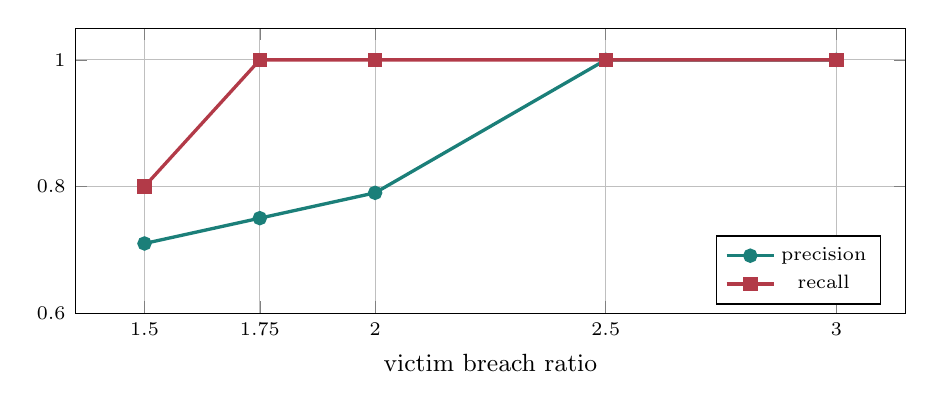
\begin{tikzpicture}
\begin{axis}[width=\textwidth, height=5.2cm, xlabel={victim breach ratio}, ymin=0.6, ymax=1.05,
  xtick={1.5,1.75,2.0,2.5,3.0}, legend pos=south east, legend style={font=\scriptsize},
  tick label style={font=\scriptsize}, label style={font=\small}, grid=major]
\addplot[teal, mark=*, very thick] coordinates {(1.5,0.71)(1.75,0.75)(2.0,0.79)(2.5,1.0)(3.0,1.0)};
\addplot[brick, mark=square*, very thick] coordinates {(1.5,0.80)(1.75,1.0)(2.0,1.0)(2.5,1.0)(3.0,1.0)};
\legend{precision,recall}
\end{axis}
\end{tikzpicture}

\scriptsize post-hoc replay of the sweep's latency data
\column{0.48\textwidth}
\small
\textbf{Fresh live run at 2.5$\times$}\par\vspace{1mm}
\begin{tabular}{lcc}
\toprule
 & pressure-only & \textbf{fused}\\
\midrule
FP idle/busy & 0/2 & \textbf{0/0}\\
Precision & 0.88 & \textbf{1.00}\\
Recall & 0.93 & 0.87\\
Latency & 14.5\,s & \textbf{2.5\,s}\\
\bottomrule
\end{tabular}
\vspace{2mm}

\normalsize
\alert{No false alarms, $\sim$6$\times$ faster}, for a small recall cost. Threshold was chosen post hoc, so we confirmed it on independent runs.
\end{columns}
\end{frame}

\begin{frame}{Evaluation bugs found and fixed}
\small
\begin{itemize}
\item \textbf{No victim effect:} node CPU pin, co-located and scaled hogs.
\item \textbf{Edge-triggered QoS events:} one event per breach onset $\Rightarrow$ re-emit while sustained; 45\,s cooldown after fairness runs.
\item \textbf{Merged alerts hid detections:} a ``both'' alert's start time came from unrelated earlier fairness evidence, scoring it a miss. Now per-track onsets: isolation 22/25 $\to$ \alert{25/25}.
\item \textbf{Meaningless metric:} ``correlation overhead'' (about 330\,s) was just time-to-scoring; replaced by measured runtime ($\approx$0.02\,s).
\item \textbf{Flaky tooling:} \texttt{grep -q} + \texttt{pipefail} intermittently aborted bring-up.
\end{itemize}
\end{frame}

\begin{frame}{Limitations (stated up front)}
\begin{itemize}
\item \textbf{2 of 15 fairness runs still missed:} resource monitor never reached its 85\% threshold; or an earlier breach merged in and started before the window.
\item \textbf{Post-hoc threshold}, confirmed on one fresh run; 15 runs per condition means wide intervals.
\item \textbf{Engineered contention}, single host, one trivial victim workload.
\item \textbf{Unaccounted alerts} aren't counted as false positives; not yet audited.
\item Auto-remediation: accepted stretch goal, \alert{not implemented}.
\end{itemize}
\end{frame}

\begin{frame}{Conclusion}
\begin{block}{Takeaways}
\begin{itemize}
\item \textbf{Isolation:} fusing control-plane and network-flow evidence detects \alert{25/25} injections with no false positives (vs.\ 0.60 / 0.40 alone).
\item \textbf{Fairness:} a victim-side breach requirement removes false alarms on busy tenants and detects \alert{$\sim$6$\times$} sooner, at a small recall cost.
\item \textbf{Honesty matters:} our first result was 0/15; the analysis that explained it is part of the contribution.
\end{itemize}
\end{block}
\textbf{Future work:} cross-validated thresholds, multi-node and realistic victim workloads, auditing unaccounted alerts, remediation.
\end{frame}

\begin{frame}[plain]
\vfill\centering
{\color{navy}\Huge\bfseries Thank you}\par\vspace{4mm}
{\color{teal}\rule{0.3\textwidth}{1.5pt}}\par\vspace{4mm}
\large Questions?\par\vfill
\end{frame}

\end{document}
